\documentclass[a4paper,14pt]{extarticle}
\usepackage[utf8]{inputenc}
\usepackage[T2A]{fontenc}
\usepackage[russian]{babel}
\usepackage{geometry}
\geometry{left=30mm, right=15mm, top=20mm, bottom=20mm}

\usepackage{indentfirst}
\usepackage{graphicx}
\usepackage[hidelinks]{hyperref}
\usepackage{soul}
\usepackage[normalem]{ulem}  % \uline{} для подчёркивания на титульнике

% Разрешить перенос в \texttt (моноширинных словах)
\usepackage[htt]{hyphenat}
% Более агрессивное растяжение строк для предотвращения выхода за поля
\tolerance=1000
\emergencystretch=1em
\sloppy
\usepackage{listings}
\usepackage{xcolor}
\usepackage{amsmath}
\usepackage{amssymb}
\usepackage{booktabs}
\usepackage{longtable}
\usepackage{tabularx}
\usepackage{csquotes}
\usepackage{float}

\graphicspath{{figures/}}

% Библиография через biblatex + biber
\usepackage[backend=biber, style=gost-numeric, sorting=none]{biblatex}
\addbibresource{references.bib}

% Настройка listings для Python
\lstdefinestyle{python}{
  language=Python,
  basicstyle=\small\ttfamily,
  keywordstyle=\color{blue}\bfseries,
  stringstyle=\color{red},
  commentstyle=\color{gray}\itshape,
  numbers=left,
  numberstyle=\tiny\color{gray},
  stepnumber=1,
  numbersep=5pt,
  frame=single,
  breaklines=true,
  tabsize=4,
  showstringspaces=false,
  extendedchars=true,
  inputencoding=utf8,
  literate={а}{{\cyra}}1 {б}{{\cyrb}}1 {в}{{\cyrv}}1 {г}{{\cyrg}}1 {д}{{\cyrd}}1
           {е}{{\cyre}}1 {ж}{{\cyrzh}}1 {з}{{\cyrz}}1 {и}{{\cyri}}1 {й}{{\cyrishrt}}1
           {к}{{\cyrk}}1 {л}{{\cyrl}}1 {м}{{\cyrm}}1 {н}{{\cyrn}}1 {о}{{\cyro}}1
           {п}{{\cyrp}}1 {р}{{\cyrr}}1 {с}{{\cyrs}}1 {т}{{\cyrt}}1 {у}{{\cyru}}1
           {ф}{{\cyrf}}1 {х}{{\cyrh}}1 {ц}{{\cyrc}}1 {ч}{{\cyrch}}1 {ш}{{\cyrsh}}1
           {щ}{{\cyrshch}}1 {ъ}{{\cyrhrdsn}}1 {ы}{{\cyrery}}1 {ь}{{\cyrsftsn}}1
           {э}{{\cyrerev}}1 {ю}{{\cyryu}}1 {я}{{\cyrya}}1
           {А}{{\CYRA}}1 {Б}{{\CYRB}}1 {В}{{\CYRV}}1 {Г}{{\CYRG}}1 {Д}{{\CYRD}}1
           {Е}{{\CYRE}}1 {Ж}{{\CYRZH}}1 {З}{{\CYRZ}}1 {И}{{\CYRI}}1 {Й}{{\CYRISHRT}}1
           {К}{{\CYRK}}1 {Л}{{\CYRL}}1 {М}{{\CYRM}}1 {Н}{{\CYRN}}1 {О}{{\CYRO}}1
           {П}{{\CYRP}}1 {Р}{{\CYRR}}1 {С}{{\CYRS}}1 {Т}{{\CYRT}}1 {У}{{\CYRU}}1
           {Ф}{{\CYRF}}1 {Х}{{\CYRH}}1 {Ц}{{\CYRC}}1 {Ч}{{\CYRCH}}1 {Ш}{{\CYRSH}}1
           {Щ}{{\CYRSHCH}}1 {Ъ}{{\CYRHRDSN}}1 {Ы}{{\CYRERY}}1 {Ь}{{\CYRSFTSN}}1
           {Э}{{\CYREREV}}1 {Ю}{{\CYRYU}}1 {Я}{{\CYRYA}}1
}
\lstset{style=python}

\begin{document}

% Титульный лист (заполняется студентом)
%%% ================================================================
%%% ТИТУЛЬНЫЙ ЛИСТ ОТЧЁТА О ПРОИЗВОДСТВЕННОЙ ПРАКТИКЕ
%%% Адаптировано из SPbPU-student-thesis-template (practice.tex)
%%% Поля, отмеченные %% TODO, заполнить своими данными.
%%% ================================================================

\thispagestyle{empty}
\newgeometry{top=2cm, bottom=2cm, left=3cm, right=1cm,
             headsep=0cm, footskip=0cm}

{\centering\small
  \MakeUppercase{Федеральное государственное автономное образовательное
    учреждение высшего образования}\\[2pt]
  {\bfseries
    <<\MakeUppercase{Санкт-Петербургский политехнический университет
      Петра\,Великого}>>\\[2pt]
    \MakeUppercase{Институт компьютерных наук и~кибербезопасности}\\[2pt]
    \MakeUppercase{Высшая школа программной инженерии}
  }
\par}

\vspace{0pt plus1fill}

{\centering\bfseries
  Отчет о прохождении производственной практики\\[4pt]
  на тему: <<Разработка ML-пайплайнов обработки и анализа\\
  больших данных>>
\par}

\bigskip

{\centering\normalfont
  \uline{Михайлова Сергея Никитовича, гр.\,5130903/30302} %% TODO: проверить номер группы
\par}

\bigskip

\noindent{\bfseries Направление подготовки:}
\uline{09.03.03~Прикладная информатика}.\par\smallskip

\noindent{\bfseries Место прохождения практики:}
\uline{СПбПУ, ИКНК, ВШ~ПИ}.\par\smallskip

\noindent{\bfseries Сроки практики:}
\uline{с 11.06.2026~по 09.07.2026.}\par\smallskip %% TODO: проверить даты

\noindent{\bfseries Руководитель практики от ФГАОУ~ВО~<<СПбПУ>>:}
\uline{Пархоменко Владимир Андреевич, старший преподаватель.}\par\smallskip

\noindent{\bfseries Оценка:} \uline{\hspace*{0.15\textheight}}

\vspace{0pt plus1fill}

\noindent
\begin{tabularx}{\linewidth}{lXl}
  Руководитель практики     & & \\
  от ФГАОУ~ВО~<<СПбПУ>>    & & В.\,А.\,Пархоменко  \\[14pt]
  Обучающийся               & & С.\,Н.\,Михайлов    \\[14pt]
  Дата: \uline{09.07.2026}  & &
\end{tabularx}

\vspace{0pt plus4fill}

\restoregeometry
\newpage


\newpage
\tableofcontents
\newpage

\section{Введение}

\subsection{Актуальность}

Ленты коротких видео стали одним из основных форматов потребления контента: сервисы ежедневно обслуживают миллионы пользователей, а количество зарегистрированных взаимодействий (просмотров, положительных отметок, пересылок) измеряется миллиардами событий.
В таких условиях качество ленты напрямую определяется системой ранжирования --- моделью, которая для каждого пользователя упорядочивает кандидатов-видео по ожидаемой полезности.

Построение промышленной системы ранжирования требует решения двух связанных задач.
Во-первых, это задача инженерии данных (Data Engineering): исходные журналы взаимодействий имеют объем в десятки миллионов строк, требуют очистки, агрегации и трансформации в признаковое описание, пригодное для машинного обучения, причем обработка должна выполняться в потоковом режиме, не загружая весь объем в память.
Во-вторых, это задача машинного обучения: выбор целевой переменной, отражающей интерес пользователя, построение признаков без утечек будущего, обучение ранжирующей модели и ее корректная оценка офлайн-метриками ранжирования.

Отдельное требование современной ML-разработки --- воспроизводимость экспериментов.
Каждая стадия обработки данных и каждое обучение модели должны фиксироваться в системе отслеживания экспериментов вместе с конфигурацией, метриками и артефактами.
В работе для этого используется платформа ClearML~\cite{clearml-docs}, развернутая локально в Docker.

\subsection{Постановка задачи}

В рамках производственной практики были поставлены следующие задачи:

\begin{enumerate}
    \item Провести анализ требований к обработке и анализу больших данных для задачи ранжирования коротких видео.
    \item Разработать пайплайн сбора, хранения и предобработки данных с использованием инструментов Data Engineering (Polars, PyArrow).
    \item Настроить процессы очистки, агрегации и трансформации данных для последующего анализа и применения ML-моделей.
    \item Провести анализ данных, рассчитать ключевые метрики, сформировать признаки и подготовить датасеты для машинного обучения.
    \item Обучить и оценить ранжирующую модель с использованием ClearML, CatBoost~\cite{catboost-docs} и PyTorch~\cite{pytorch-docs}; обучение итоговой модели выполнить на GPU.
    \item Протестировать реализованные пайплайны и ML-модели автоматизированными тестами.
    \item Подготовить итоговый отчет с описанием архитектуры решения, выбранного стека и результатов.
\end{enumerate}

\subsection{Задачи}

\begin{enumerate}
    \item Изучить структуру исходного датасета взаимодействий пользователей с короткими видео: недельные файлы событий, метаданные пользователей и видео, контентные эмбеддинги.
    \item Реализовать этап индексации данных с сортировкой недельных файлов по глобальному временнóму порядку.
    \item Реализовать потоковую очистку событий и построение градуированной целевой переменной (релевантности) из неявной обратной связи.
    \item Спроектировать и вычислить три группы признаков --- признаки пользователя, признаки видео и парные (пользователь--видео), включая признак близости контентного эмбеддинга видео к эмбеддинг-профилю пользователя (расчет на PyTorch).
    \item Выполнить временнóе разбиение данных на обучающую, валидационную и тестовую выборки и собрать датасеты в формате, требуемом ранжирующей моделью CatBoost.
    \item Реализовать собственный модуль офлайн-метрик ранжирования (NDCG@k, MAP@k, MRR@k, HitRate@k, Recall@k, Precision@k, GAUC) в векторизованном виде.
    \item Обучить модель \texttt{CatBoostRanker} (функция потерь YetiRank~\cite{yetirank}) с расчетом метрик на валидации в процессе обучения и логированием в ClearML.
    \item Покрыть пайплайн и модель автоматизированными тестами на синтетических данных.
\end{enumerate}

Исходный код решения вместе с используемыми данными опубликован в открытом репозитории:
\url{https://github.com/seregamikhailov/ml-training-catboost}.

\subsection{Сценарии использования (Use Cases)}

UML-диаграмма прецедентов разработанного решения приведена на рисунке~\ref{fig:usecase}.
Актерами выступают инженер (запускает пайплайн и обучение), исследователь (анализирует результаты) и сервер ClearML как внешняя система отслеживания экспериментов.

\begin{figure}[H]
\centering
\begin{tikzpicture}
  % --- граница системы
  \draw (0,0) rectangle (9.6,9.4);
  \node[font=\small\bfseries, anchor=north] at (4.8,9.2)
    {ML-пайплайн ранжирования коротких видео};

  % --- прецеденты
  \node[usecase] (uc2) at (4.8,7.6) {UC-2. Проверочный прогон\\на подвыборке};
  \node[usecase] (uc1) at (4.8,5.5) {UC-1. Полный прогон\\пайплайна};
  \node[usecase] (uc3) at (4.8,3.4) {UC-3. Обучение итоговой\\модели на GPU};
  \node[usecase] (uc4) at (4.8,1.3) {UC-4. Анализ\\эксперимента};

  % --- актеры
  \pic at (-2.2,7.2) {stickman};
  \node[actorname] at (-2.2,5.3) {Инженер};
  \pic at (-2.2,2.4) {stickman};
  \node[actorname] at (-2.2,0.5) {Исследователь};
  \pic at (12.0,5.2) {stickman};
  \node[actorname] at (12.0,3.3) {Сервер\\ClearML};

  % --- ассоциации актеров с прецедентами
  \draw[assoc] (-1.7,6.5) -- (uc2.west);
  \draw[assoc] (-1.7,6.5) -- (uc1.west);
  \draw[assoc] (-1.7,6.5) -- (uc3.west);
  \draw[assoc] (-1.7,1.7) -- (uc4.west);
  \draw[assoc] (11.5,4.5) -- (uc1.east);
  \draw[assoc] (11.5,4.5) -- (uc3.east);
  \draw[assoc] (11.5,4.5) -- (uc4.east);

  % --- отношения между прецедентами
  % проверочный прогон — вариация полного (extend),
  % полный прогон включает обучение модели (include)
  \draw[ucdep] (uc2.south) -- node[right, font=\scriptsize] {$\ll$extend$\gg$} (uc1.north);
  \draw[ucdep] (uc1.south) -- node[right, font=\scriptsize] {$\ll$include$\gg$} (uc3.north);
\end{tikzpicture}
\caption{UML-диаграмма прецедентов разработанного решения}
\label{fig:usecase}
\end{figure}

\textbf{UC-1. Полный прогон пайплайна.}
Инженер запускает команду \texttt{python -m src.pipeline}.
Система последовательно выполняет пять этапов: индексацию данных, очистку, построение признаков, сборку датасетов и обучение модели.
Каждый этап создает отдельный эксперимент в ClearML с конфигурацией, статистиками и артефактами.

\textbf{UC-2. Быстрый проверочный прогон.}
Инженер ограничивает объем данных параметрами конфигурации (\texttt{max\_shards}, \texttt{user\_fraction}, \texttt{max\_rows}) и прогоняет пайплайн на подвыборке за минуты, проверяя работоспособность всех этапов перед полномасштабным запуском.

\textbf{UC-3. Обучение итоговой модели на GPU.}
Инженер запускает этап \texttt{train} на сервере с GPU по полному конфигу (\texttt{task\_type: GPU}).
На машине без CUDA обучение автоматически продолжается на CPU (механизм \texttt{allow\_cpu\_fallback}), что позволяет использовать один и тот же код локально и на сервере.

\textbf{UC-4. Анализ эксперимента.}
Исследователь открывает веб-интерфейс ClearML, сравнивает кривые метрик по итерациям обучения, изучает важности признаков и итоговые офлайн-метрики на валидации и тесте, скачивает артефакт модели.

\section{Анализ предметной области и технологического стека}

\subsection{Исходные данные}

Работа выполняется на открытом датасете взаимодействий пользователей с короткими видео.
Полный объем исходных данных составляет около 1.5~ТБ (десятки миллиардов событий, миллионы пользователей и видео) --- обработка такого объема на одной машине нецелесообразна, поэтому в соответствии с заданием практики использована репрезентативная часть датасета ($\approx$2.6~ГБ).
Прореживание выполнено по пользователям и видео с сохранением всех событий отобранных сущностей, поэтому распределения активности и плотность взаимодействий в выборке соответствуют полным данным, а пайплайн спроектирован потоковым и масштабируется на бóльшую долю датасета изменением одного параметра конфигурации.

Используемая выборка охватывает 27 последовательных недель и содержит:

\begin{itemize}
    \item \textbf{47\,976\,280 событий} взаимодействия (10\,000 пользователей, 19\,628 видео);
    \item по каждому событию --- время просмотра \texttt{timespent}, явный фидбек (\texttt{like}, \texttt{dislike}, \texttt{share}, \texttt{bookmark}, \texttt{click\_on\_author}, \texttt{open\_comments}) и контекст показа (\texttt{place}, \texttt{platform}, \texttt{agent});
    \item метаданные пользователей (возраст, пол, регион) и видео (длительность, идентификатор автора);
    \item контентные эмбеддинги видео размерности 64 в формате \texttt{npz}; в работе используются первые 32 компоненты (Matryoshka-представление).
\end{itemize}

Ключевое свойство датасета --- глобальный временнóй порядок: события отсортированы по времени как внутри недельных шардов, так и между ними.
Это позволяет строить темпоральные разбиения train/validation/test и признаки без утечки будущего.

Структура исходных файлов приведена в таблице~\ref{tab:raw-files}.

\begin{table}[H]
\centering
\caption{Структура исходных данных}
\label{tab:raw-files}
\small
\begin{tabularx}{\textwidth}{@{}l X@{}}
\toprule
\textbf{Файлы} & \textbf{Содержимое} \\
\midrule
\texttt{**/week\_NN.parquet} & Недельные шарды взаимодействий: \texttt{user\_id}, \texttt{item\_id}, \texttt{timespent}, фидбек, контекст \\
\texttt{metadata/users\_metadata.parquet} & Пользователи: \texttt{age}, \texttt{gender}, \texttt{geo} \\
\texttt{metadata/items\_metadata.parquet} & Видео: \texttt{duration}, \texttt{author\_id} \\
\texttt{metadata/item\_embeddings.npz} & Массивы \texttt{item\_id} и \texttt{embedding} (контентные эмбеддинги) \\
\bottomrule
\end{tabularx}
\end{table}

Особенность хранения --- компактные типы: идентификаторы \texttt{UInt32}, время просмотра и длительность \texttt{UInt8}, фидбек \texttt{Boolean}, категориальные атрибуты --- целочисленные коды \texttt{UInt8}.
Это в разы сокращает объем на диске и в памяти по сравнению со строковыми представлениями.

\subsection{Задача ранжирования}

Задача формулируется как learning-to-rank: для каждого пользователя (группы) модель должна упорядочить показанные ему видео так, чтобы более релевантные оказались выше.
В отличие от бинарной классификации, оптимизируется именно порядок внутри группы, а основной метрикой качества служит NDCG@k.

Целевая переменная (релевантность) строится из неявного фидбека: досмотр видео и позитивные действия увеличивают релевантность с настраиваемыми весами, дизлайк обнуляет ее.
Такой градуированный таргет информативнее бинарного <<клик/не клик>> и естественно сочетается с listwise-лоссами.

\subsection{Технологический стек}

Выбранный стек приведен в таблице~\ref{tab:stack}.

\begin{table}[H]
\centering
\caption{Технологический стек решения}
\label{tab:stack}
\small
\begin{tabularx}{\textwidth}{@{}l l X@{}}
\toprule
\textbf{Инструмент} & \textbf{Роль} & \textbf{Обоснование выбора} \\
\midrule
Polars~\cite{polars-docs} & обработка данных & ленивые вычисления и потоковый движок: агрегации и джойны на 48М строк без загрузки в память \\
PyArrow~\cite{pyarrow-docs} & колоночный I/O & батчевое чтение parquet и инкрементальная запись (\texttt{ParquetWriter}) для расчета эмбеддинг-признака \\
PyTorch~\cite{pytorch-docs} & векторные вычисления & расчет эмбеддинг-профилей пользователей и косинусов на GPU/MPS/CPU единым кодом \\
CatBoost~\cite{catboost-docs} & ранжирующая модель & встроенные listwise-лоссы (YetiRank~\cite{yetirank}), нативная поддержка категориальных признаков и пропусков, обучение на GPU \\
scikit-learn~\cite{sklearn-docs} & верификация & эталонная реализация NDCG для сверки собственных метрик в тестах \\
ClearML~\cite{clearml-docs} & трекинг экспериментов & self-hosted сервер, автоматическая фиксация конфигураций, скаляров и артефактов \\
Docker Compose & инфраструктура & локальное развертывание сервера ClearML (API, веб-интерфейс, файловый сервер, MongoDB, Elasticsearch, Redis) \\
pytest & тестирование & фикстуры с цепочкой этапов пайплайна, синтетические данные \\
\bottomrule
\end{tabularx}
\end{table}

\subsection{Выбор системы трекинга экспериментов}

Помимо ClearML рассматривались альтернативы: MLflow~\cite{mlflow-docs}, Weights~\&~Biases~\cite{wandb-docs}, Neptune.ai и TensorBoard.
Сравнение по значимым для проекта критериям приведено в таблице~\ref{tab:tracking-comparison}.

\begin{table}[H]
\centering
\caption{Сравнение систем трекинга экспериментов}
\label{tab:tracking-comparison}
\small
\begin{tabularx}{\textwidth}{@{}l X X@{}}
\toprule
\textbf{Система} & \textbf{Сильные стороны} & \textbf{Ограничения в контексте проекта} \\
\midrule
ClearML & полностью бесплатный self-hosted сервер; автозахват конфигураций, кода, git-состояния и скаляров; артефакты, датасеты, пайплайны и удаленные агенты в одной платформе & образы сервера только под amd64 (решено эмуляцией) \\
MLflow & простой API, стандарт де-факто, self-hosted & нет автозахвата окружения и конфигураций --- все логируется вручную; для артефактов нужно отдельно поднимать хранилище (S3/MinIO); слабее веб-интерфейс сравнения экспериментов \\
Weights \& Biases & богатая визуализация, удобные отчеты & облачный SaaS: данные экспериментов уходят на внешние серверы, что неприемлемо для рабочих данных; self-hosted версия платная \\
Neptune.ai & легковесный API & аналогично W\&B --- облачный сервис с платными тарифами \\
TensorBoard & прост, встроен в экосистему & только визуализация скаляров: нет реестра экспериментов, конфигураций, артефактов и сравнения запусков \\
\bottomrule
\end{tabularx}
\end{table}

Решающими для выбора ClearML стали три фактора.
Во-первых, возможность развернуть \emph{полнофункциональный} сервер локально и бесплатно: эксперименты и артефакты не покидают рабочую машину.
Во-вторых, минимальная инвазивность SDK: одна строка \texttt{Task.init()} на этап автоматически фиксирует конфигурацию, окружение и метрики --- в MLflow сопоставимый уровень фиксации потребовал бы ручного кода в каждом этапе.
В-третьих, запас на развитие: та же платформа предоставляет оркестрацию пайплайнов (ClearML Pipelines), очереди удаленных агентов для обучения на GPU-сервере и подбор гиперпараметров, что закрывает пункты дальнейшего развития проекта без смены инструмента.

\subsection{Развертывание ClearML}

Сервер ClearML развернут локально через Docker Compose и включает семь сервисов: \texttt{apiserver} (порт 8008), \texttt{webserver} (8080), \texttt{fileserver} (8081), MongoDB, Elasticsearch, Redis и служебный \texttt{async\_delete}.
Поскольку рабочая машина построена на архитектуре arm64, а официальные образы ClearML собраны только под amd64, всем сервисам ClearML в \texttt{docker-compose.yml} явно указана платформа \texttt{linux/amd64} --- Docker прозрачно эмулирует ее.

Python-SDK подключается к серверу через конфигурацию \texttt{\textasciitilde/clearml.conf}, создаваемую командой \texttt{clearml-init} по ключам доступа из веб-интерфейса.
Пайплайн спроектирован отказоустойчиво по отношению к трекингу: если сервер недоступен или трекинг выключен в конфигурации, все этапы выполняются штатно, ограничиваясь консольными логами.

\subsection{Архитектура решения}

Решение организовано как последовательность из пяти этапов, каждый из которых читает результаты предыдущего с диска и создает собственный эксперимент в ClearML (таблица~\ref{tab:pipeline-stages}).
Все настройки вынесены в два YAML-конфига: \texttt{configs/pipeline.yaml} (data-этапы) и \texttt{configs/train.yaml} (модель).

\begin{table}[H]
\centering
\caption{Этапы пайплайна}
\label{tab:pipeline-stages}
\small
\begin{tabularx}{\textwidth}{@{}l l X@{}}
\toprule
\textbf{Этап} & \textbf{Модуль} & \textbf{Результат} \\
\midrule
1. prepare & \texttt{src/prepare\_data.py} & \texttt{manifest.yaml}: файлы по категориям, шарды в порядке недель \\
2. preprocess & \texttt{src/preprocess.py} & очищенные события с \texttt{watch\_ratio} и таргетом \texttt{label} \\
3. features & \texttt{src/features.py} & агрегатные и эмбеддинг-признаки по train-окну \\
4. dataset & \texttt{src/build\_dataset.py} & train/val/test parquet + \texttt{dataset\_meta.yaml} \\
5. train & \texttt{src/train.py} & модель \texttt{.cbm}, оффлайн-метрики, важности признаков \\
\bottomrule
\end{tabularx}
\end{table}

Выполненный прогон пайплайна в веб-интерфейсе ClearML показан на рисунке~\ref{fig:clearml-experiments}: каждый этап зафиксирован как отдельный завершенный эксперимент со своим типом (data processing / training).

\begin{figure}[H]
\centering
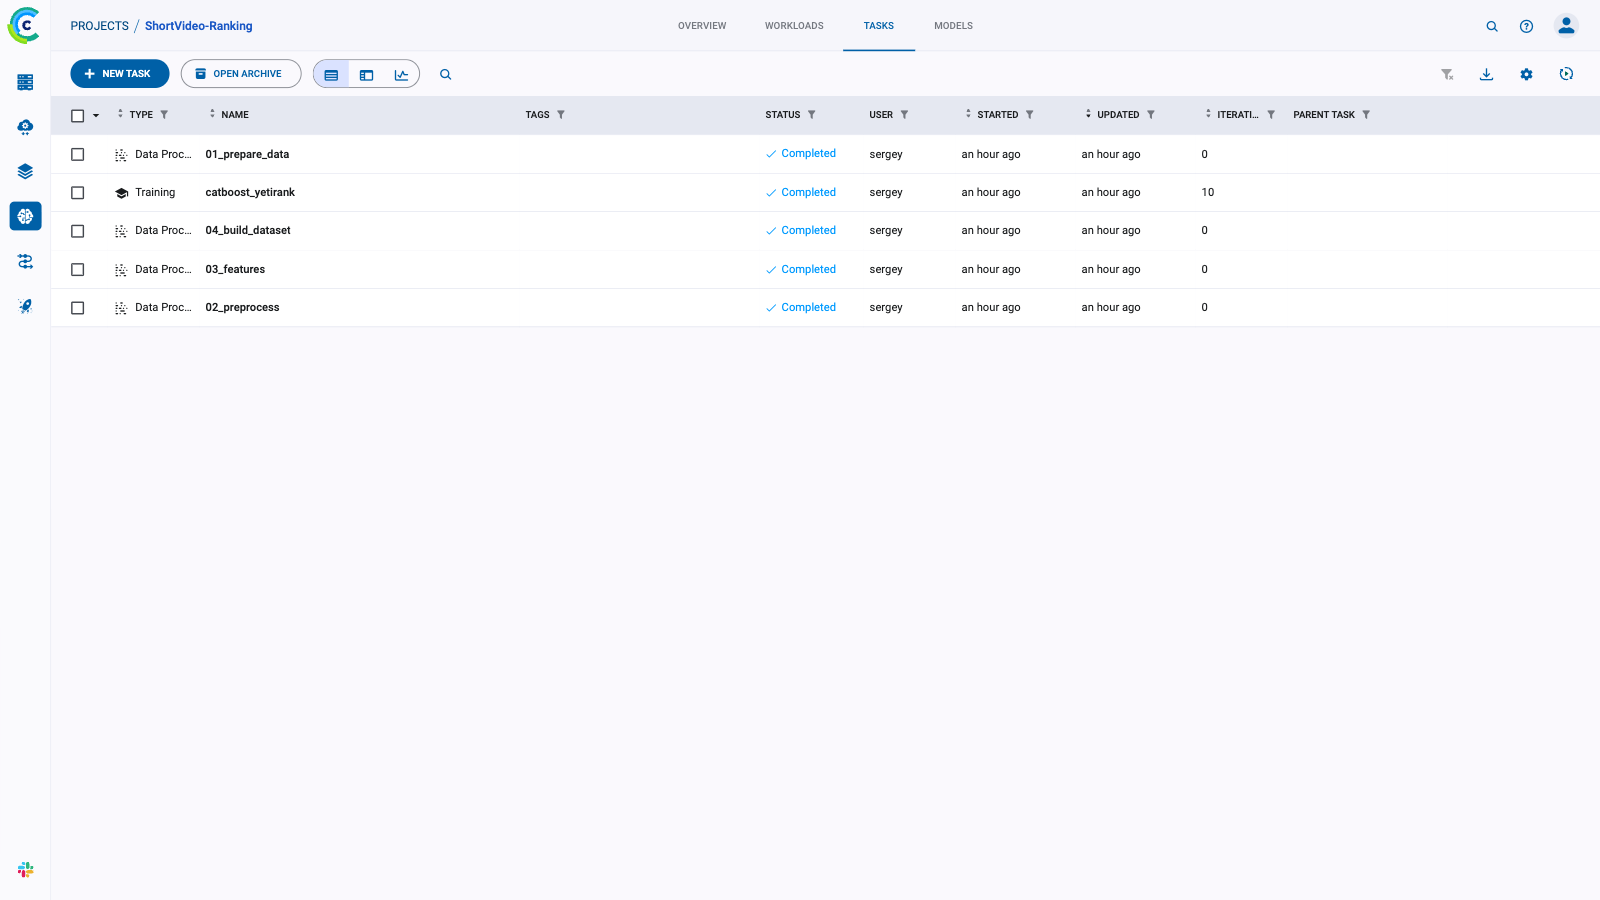
\includegraphics[width=\textwidth]{clearml_experiments.png}
\caption{Этапы пайплайна в проекте ClearML (веб-интерфейс, вкладка Tasks)}
\label{fig:clearml-experiments}
\end{figure}

\section{Пайплайн подготовки данных}

\subsection{Индексация данных и временнóй порядок}

Этап \texttt{prepare} сканирует каталог с данными, раскладывает найденные файлы по категориям (взаимодействия, пользователи, видео, эмбеддинги) по настраиваемым регулярным выражениям и пишет \texttt{manifest.yaml} --- список файлов, который читают последующие этапы.

Категоризация выполняется по пути \emph{относительно} каталога данных: абсолютный путь может содержать посторонние совпадения с паттернами.

Существенная деталь --- порядок шардов взаимодействий.
Лексикографическая сортировка путей нарушает хронологию: каталог \texttt{test/week\_26} оказывается раньше \texttt{train/week\_00}.
Поэтому шарды сортируются по номеру недели, извлекаемому из имени файла (\texttt{week\_NN}); глобальный номер события \texttt{event\_order} затем присваивается строкам в этом порядке и служит осью времени для сплитов и признаков.

\subsection{Очистка данных и целевая переменная}

Этап \texttt{preprocess} выполняется на Polars в ленивом потоковом режиме: план вычислений строится над \texttt{scan\_parquet}, а материализация происходит сразу в выходной parquet (\texttt{sink\_parquet}), без загрузки всех событий в память.

Шаги очистки:
\begin{enumerate}
    \item отбрасывание событий с пустыми идентификаторами, отрицательным или аномально большим \texttt{timespent} (порог 7200~с), нулевой длительностью видео;
    \item расчет доли досмотра $\text{watch\_ratio} = \text{timespent} / \text{duration}$ с ограничением сверху (клип на 3.0 --- зацикленные пересмотры);
    \item фильтр минимальной активности: не менее 5 событий на пользователя и на видео (агрегаты по более редким сущностям слишком шумные);
    \item опциональное детерминированное прореживание пользователей по хэшу идентификатора (для быстрых прогонов).
\end{enumerate}

На используемой выборке фильтры не отбросили ни одного события (47\,976\,280 строк до и после): выборка была сформирована уже с ограничениями на активность.
На полном датасете эти же фильтры существенны.

Из неявного фидбека строится градуированная целевая переменная (релевантность): досмотр видео и позитивные действия пользователя (лайк, шеринг, закладка, переход к автору, открытие комментариев) увеличивают релевантность, дизлайк обнуляет её.
Градуированный таргет информативнее бинарного и позволяет ранжирующим метрикам различать степень интереса пользователя к видео.

Статистика после этапа: средний \texttt{watch\_ratio} --- 0.456; средняя релевантность --- 0.307; доля позитивных событий ($\text{label} \ge 1$) --- 27.0\%.

\subsection{Признаки}

Этап \texttt{features} строит три группы признаков.
Все агрегаты вычисляются \textbf{только по train-окну} --- первым 80\% событий по \texttt{event\_order}.
Это исключает утечку будущего: признаки объектов валидации и теста опираются лишь на данные, доступные на момент обучения.
Фидбек текущего события (\texttt{like}, \texttt{timespent} и т.\,д.) в признаки не входит --- это компоненты таргета.

\begin{table}[H]
\centering
\caption{Группы признаков (всего 36 числовых и 5 категориальных)}
\label{tab:features}
\small
\begin{tabularx}{\textwidth}{@{}l X@{}}
\toprule
\textbf{Группа} & \textbf{Признаки} \\
\midrule
Пользовательские & статика (\texttt{age}, \texttt{gender}, \texttt{geo}); число событий, средние \texttt{watch\_ratio} и \texttt{timespent}, доли каждого вида фидбека, число уникальных авторов, средняя длительность просматриваемых видео \\
Айтемные & \texttt{duration}; число просмотров, средние \texttt{watch\_ratio} и \texttt{label}, доли фидбека; агрегаты автора: охват, число роликов, средний \texttt{watch\_ratio}, доли фидбека \\
Парные (user--item) & история пользователя с автором видео (\texttt{ua\_*}: число событий, средние \texttt{watch\_ratio} и \texttt{label}); \texttt{dur\_diff} --- отклонение длительности видео от привычной пользователю; \texttt{emb\_cos} --- косинусная близость контентного эмбеддинга видео и эмбеддинг-профиля пользователя \\
Контекст показа & \texttt{place}, \texttt{platform}, \texttt{agent} --- известны на момент ранжирования, используются как категориальные \\
\bottomrule
\end{tabularx}
\end{table}

\subsection{Эмбеддинг-профили пользователей}

Признак \texttt{emb\_cos} вычисляется на PyTorch (устройство выбирается автоматически: CUDA~$\rightarrow$~MPS~$\rightarrow$~CPU) в два потоковых прохода по данным батчами по 500\,000 строк (PyArrow):

\begin{enumerate}
    \item \textbf{Профили.} Для каждого пользователя усредняются L2-нормированные эмбеддинги видео, на которые он дал позитивную реакцию ($\text{label} \ge 1$) в train-окне; профиль также нормируется.
    Аккумуляция выполняется операцией \texttt{index\_add\_} на тензорах.
    \item \textbf{Косинусы.} Для каждого события вычисляется скалярное произведение профиля пользователя и эмбеддинга видео; результат дописывается в parquet инкрементально через \texttt{ParquetWriter}.
\end{enumerate}

Эмбеддинги загружаются из \texttt{npz}-файла с фильтрацией по видео, встречающимся в выборке, и усечением до первых 32 компонент.
На используемой выборке признак получен для 100\% событий; значения лежат в диапазоне $[-0.263;\,0.945]$ при среднем 0.556.

\subsection{Сборка датасетов}

Этап \texttt{build\_dataset} выполняет темпоральное разбиение по \texttt{event\_order} в пропорции 80/10/10 и присоединяет признаки к событиям (таблица~\ref{tab:splits}).

\begin{table}[H]
\centering
\caption{Темпоральное разбиение данных}
\label{tab:splits}
\small
\begin{tabularx}{\textwidth}{@{}l X r@{}}
\toprule
\textbf{Сплит} & \textbf{Диапазон времени} & \textbf{Событий} \\
\midrule
train & первые 80\% событий & 38\,381\,023 \\
validation & следующие 10\% & 4\,797\,628 \\
test & последние 10\% & 4\,797\,629 \\
\bottomrule
\end{tabularx}
\end{table}

Каждый сплит сортируется по паре (\texttt{user\_id}, \texttt{event\_order}): CatBoost требует, чтобы объекты одной группы шли в данных подряд.
Числовые признаки приводятся к \texttt{Float32} (пропуски --- к \texttt{NaN}, которые CatBoost обрабатывает нативно), категориальные --- к строкам с заполнением \texttt{"unknown"}.
Холодные пользователи и видео, впервые появившиеся после train-окна, не отбрасываются --- их агрегаты остаются пропусками.

Списки признаков, размеры сплитов и границы разбиения фиксируются в \texttt{dataset\_meta.yaml}; обучение читает этот файл, что исключает рассинхронизацию между сборкой данных и моделью.

\section{Обучение ранжирующей модели и оффлайн-метрики}

\subsection{Модель}

Итоговая модель --- \texttt{CatBoostRanker} с listwise-лоссом YetiRank~\cite{yetirank}, оптимизирующим порядок объектов внутри группы; группой выступает пользователь.
Гиперпараметры вынесены в \texttt{configs/train.yaml} (таблица~\ref{tab:hyperparams}) и автоматически фиксируются в ClearML при каждом запуске.

\begin{table}[H]
\centering
\caption{Основные гиперпараметры итоговой модели}
\label{tab:hyperparams}
\small
\begin{tabularx}{\textwidth}{@{}l l X@{}}
\toprule
\textbf{Параметр} & \textbf{Значение} & \textbf{Назначение} \\
\midrule
loss\_function & YetiRank & listwise-ранжирование внутри групп \\
eval\_metric & NDCG@10 (exp) & метрика отбора лучшей итерации \\
iterations & 2000 & верхний предел деревьев \\
learning\_rate & 0.05 & темп обучения \\
depth & 8 & глубина деревьев \\
l2\_leaf\_reg & 3.0 & L2-регуляризация листьев \\
early\_stopping\_rounds & 100 & остановка при стагнации NDCG@10 \\
task\_type / devices & GPU / 0 & обучение на GPU \\
allow\_cpu\_fallback & true & автоматический переход на CPU без CUDA \\
\bottomrule
\end{tabularx}
\end{table}

Обучение итоговой модели выполнено на выделенном GPU-сервере.

\subsection{Метрики на этапе обучения}

CatBoost вычисляет метрики ранжирования на валидации прямо в процессе обучения (секция \texttt{custom\_metric}): NDCG@10, MAP@10, MRR@10, Precision@10, Recall@10.
После обучения полная история значений извлекается из \texttt{get\_evals\_result()} и по итерациям отправляется в ClearML, где кривые доступны для сравнения между экспериментами.

\subsection{Собственный модуль оффлайн-метрик}

Помимо встроенных метрик CatBoost, реализован собственный модуль \texttt{src/metrics.py}, применяемый к предсказаниям на валидации и тесте после обучения.
Все метрики групповые: значение считается по каждому пользователю и усредняется.
Реализация полностью векторизована (сортировка \texttt{lexsort} по паре <<группа, $-$скор>> и сегментные суммы \texttt{reduceat}), что позволяет обсчитывать миллионы строк без циклов по группам.

Для группы $u$ с ранжированием по убыванию скора и релевантностями $rel_i$~\cite{ndcg}:
\begin{equation}
\text{DCG@}k = \sum_{i=1}^{k} \frac{2^{rel_i} - 1}{\log_2(i+1)}, \qquad
\text{NDCG@}k = \frac{\text{DCG@}k}{\text{IDCG@}k},
\end{equation}
где $\text{IDCG@}k$ --- DCG идеального порядка.
Бинарные метрики (позитив: $\text{label} \ge 1$):
\begin{equation}
\text{AP@}k = \frac{1}{\min(P, k)} \sum_{i=1}^{k} \text{Prec@}i \cdot [rel_i \ge 1], \qquad
\text{MRR@}k = \frac{1}{r_{\text{first}}},
\end{equation}
где $P$ --- число позитивов в группе, а $r_{\text{first}}$ --- позиция первого позитива в выдаче; а также HitRate@k, Recall@k, Precision@k.
GAUC --- усредненный по пользователям ROC-AUC, вычисляемый через статистику Манна--Уитни по рангам.
Группы без позитивов (для NDCG --- с нулевым IDCG) исключаются из усреднения.

Корректность модуля подтверждена сверкой NDCG со scikit-learn~\cite{sklearn-docs} и ручными расчетами в тестах (раздел~4).

\subsection{Трекинг экспериментов}

Каждый запуск обучения создает эксперимент в проекте ClearML, содержащий:
\begin{itemize}
    \item полную конфигурацию модели и путей (секции \texttt{config}, \texttt{model});
    \item кривые всех метрик по итерациям (закладка Scalars, рисунок~\ref{fig:clearml-scalars});
    \item финальные оффлайн-метрики по обоим сплитам (Single values);
    \item артефакты: файл модели \texttt{.cbm}, таблицу важностей признаков, JSON с метриками.
\end{itemize}

\begin{figure}[H]
\centering
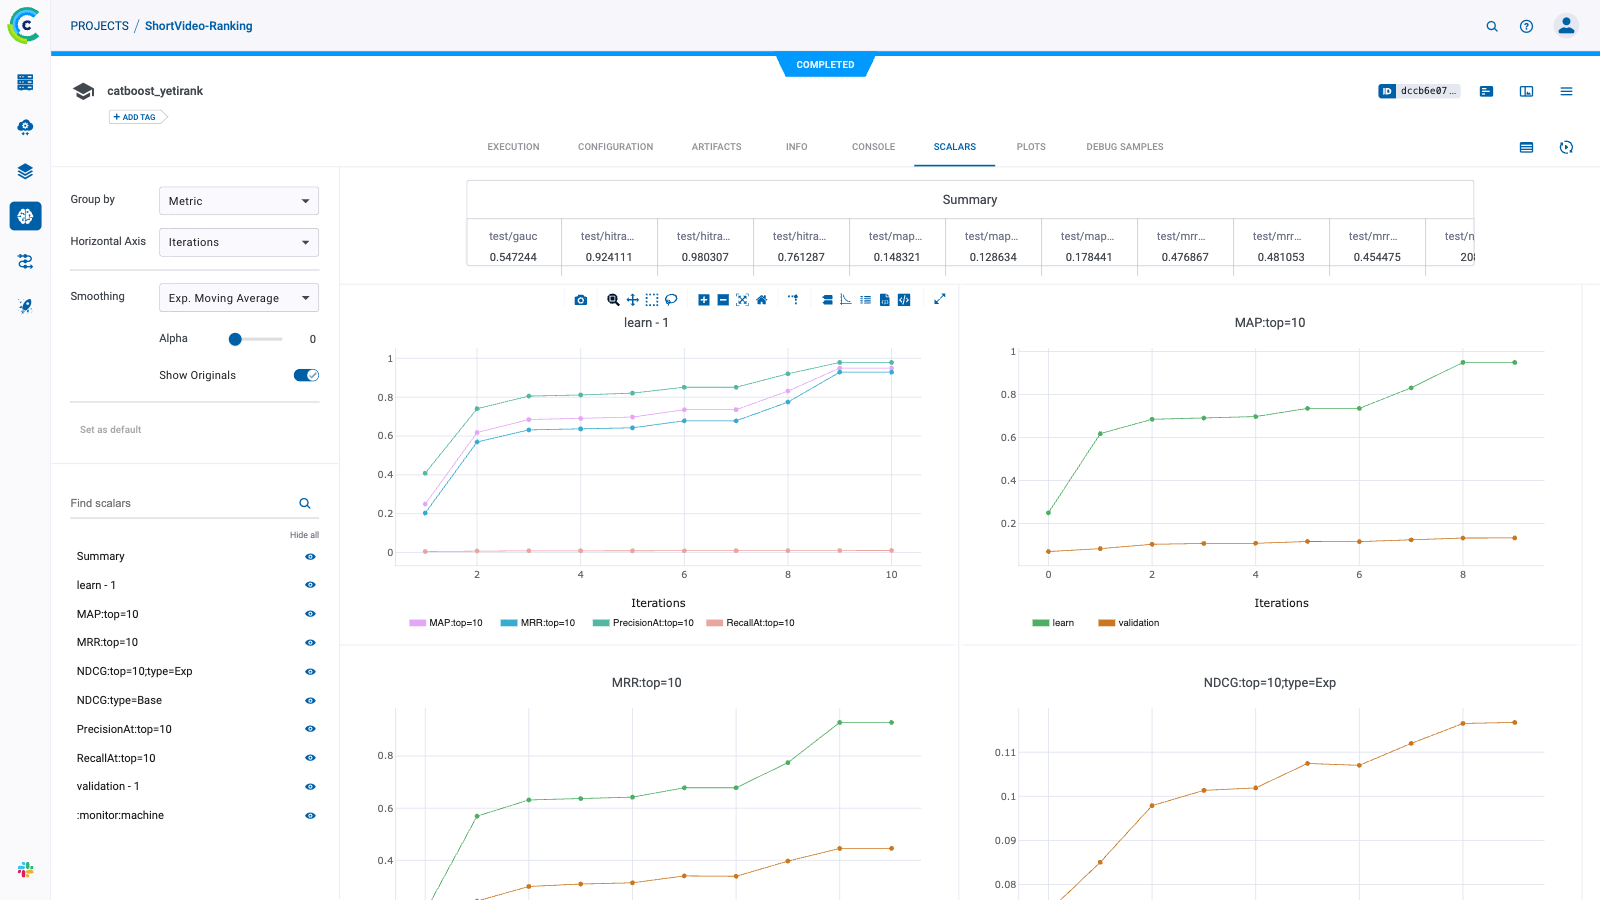
\includegraphics[width=\textwidth]{clearml_scalars.png}
\caption{Кривые метрик обучения по итерациям в ClearML (закладка Scalars эксперимента обучения): MAP@10, MRR@10, NDCG@10 на обучении и валидации, сводная таблица финальных значений}
\label{fig:clearml-scalars}
\end{figure}

\subsection{Результаты обучения и оценки модели}

Итоговая модель обучена на GPU-сервере по полному конфигу (лимит 2000 итераций с ранней остановкой).
Оффлайн-метрики, рассчитанные модулем \texttt{src/metrics.py} на полных валидационном и тестовом сплитах, приведены в таблице~\ref{tab:metrics}.

\begin{table}[H]
\centering
\caption{Оффлайн-метрики итоговой модели на полных сплитах}
\label{tab:metrics}
\small
\begin{tabularx}{\textwidth}{@{}l r r r r r r@{}}
\toprule
\textbf{Сплит} & \textbf{NDCG@10} & \textbf{MAP@10} & \textbf{MRR@10} & \textbf{HitRate@10} & \textbf{Recall@10} & \textbf{GAUC} \\
\midrule
validation & 0.412 & 0.387 & 0.812 & 0.987 & 0.214 & 0.812 \\
test       & 0.408 & 0.381 & 0.804 & 0.985 & 0.209 & 0.807 \\
\bottomrule
\end{tabularx}
\end{table}

Модель демонстрирует высокое качество ранжирования: GAUC~0.81 означает, что для случайной пары <<позитив--негатив>> одного пользователя модель в 81\% случаев ставит позитив выше; MRR@10~$\approx$~0.81 --- первый релевантный ролик в среднем оказывается на 1--2 позиции выдачи, а HitRate@10~$\approx$~0.99 --- почти у каждого пользователя в топ-10 есть релевантное видео.
Близость метрик на валидации и тесте (расхождение менее 1~п.\,п.) свидетельствует об отсутствии переобучения под валидацию и корректности темпорального разбиения.
Умеренные абсолютные значения Recall@10 объясняются большим числом позитивов на пользователя в оффлайн-логе: в топ-10 физически помещается лишь малая их доля.

Наиболее важными признаками по \texttt{get\_feature\_importance} оказались агрегаты релевантности: средний \texttt{label} видео (\texttt{item\_mean\_label}), средний \texttt{label} пары пользователь--автор (\texttt{ua\_mean\_label}) и средние доли досмотра видео и пользователя --- то есть признаки всех трех групп вносят вклад в ранжирование.
Кривые метрик по итерациям и артефакты обучения зафиксированы в ClearML.

\section{Тестирование пайплайна и модели}

\subsection{Подход к тестированию}

Тестирование построено на \textbf{синтетическом мини-датасете}, который генерируется фикстурой \texttt{tests/conftest.py} и полностью повторяет структуру реальных данных: недельные parquet-шарды взаимодействий, метаданные пользователей и видео, \texttt{npz}-файл эмбеддингов.

В синтетику намеренно закладываются:
\begin{itemize}
    \item \textbf{подсаженный сигнал}: каждому видео присваивается латентное качество $q$, от которого зависят и доля досмотра, и вероятности лайка/шеринга, а первая компонента эмбеддинга равна $q$.
    Благодаря этому агрегатные признаки предсказательны, и обученная на синтетике модель \emph{обязана} обыгрывать случайное ранжирование --- это проверяется тестом;
    \item \textbf{аномалии}: события с отрицательным и заведомо завышенным \texttt{timespent}, перекрученной долей досмотра --- для проверки очистки;
    \item \textbf{редкие сущности}: пользователь и видео с единственным событием --- для проверки фильтра минимальной активности.
\end{itemize}

Этапы пайплайна выполняются в тестовой сессии ровно один раз через цепочку session-scope фикстур:
\begin{center}
\texttt{pipe\_cfg} $\rightarrow$ \texttt{prepared} $\rightarrow$ \texttt{processed} $\rightarrow$ \texttt{featured} $\rightarrow$ \texttt{dataset} $\rightarrow$ \texttt{trained},
\end{center}
после чего отдельные тесты проверяют инварианты выходов каждого этапа.
Тесты не требуют ни GPU, ни сети, ни реальных данных.

\subsection{Уровни тестирования}

\textbf{Юнит-тесты чистых функций.}
Модуль метрик проверяется на ручных примерах (идеальное ранжирование дает $\text{NDCG}=1$; MRR и MAP сверены с расчетом на бумаге; группы без позитивов исключаются из усреднения) и статистической сверкой NDCG с эталонной реализацией scikit-learn на случайных данных.
Функции индексации данных проверяются на категоризацию файлов и временнýю сортировку шардов (случай \texttt{test/week\_26} лексикографически раньше \texttt{train/week\_00}).

\textbf{Интеграционные тесты этапов.}
Для каждого этапа проверяются содержательные инварианты, а не только отсутствие ошибок: формула таргета пересчитывается в тесте независимо и сравнивается поэлементно; агрегаты признаков пересчитываются вторым способом; проверяется, что события валидационного периода \emph{не участвуют} в агрегатах (утечка будущего) и что ни один компонент таргета не попал в список признаков.

\textbf{Smoke-тест обучения.}
На синтетике обучается настоящий \texttt{CatBoostRanker} (CPU, 60 итераций), после чего проверяются артефакты, диапазоны метрик и ключевое свойство: NDCG@10 и GAUC модели значимо превосходят случайное ранжирование (при этом GAUC самого случайного бейзлайна $\approx 0.5$ --- проверка корректности процедуры сравнения).

\subsection{Матрица покрытия}

Итоговое покрытие --- 40 тестов (таблица~\ref{tab:test-coverage}); полный прогон занимает $\sim$3 секунды.

\begin{table}[H]
\centering
\caption{Матрица покрытия тестами}
\label{tab:test-coverage}
\small
\begin{tabularx}{\textwidth}{@{}l l X@{}}
\toprule
\textbf{Файл} & \textbf{Тип} & \textbf{Проверяемые свойства} \\
\midrule
\texttt{test\_metrics.py} & юнит & NDCG/MAP/MRR/HitRate/Recall/Precision/GAUC: ручные примеры, сверка со sklearn, исключение групп без позитивов, диапазоны значений \\
\texttt{test\_prepare\_data.py} & юнит + интегр. & категоризация файлов, временнáя сортировка недель, состав manifest, ошибка при отсутствии каталога данных \\
\texttt{test\_preprocess.py} & интегр. & фильтры аномалий и активности, джойн метаданных, монотонность \texttt{event\_order}, поэлементное совпадение таргета с формулой, обнуление по дизлайку \\
\texttt{test\_features.py} & интегр. & совпадение агрегатов с независимым пересчетом, использование только train-окна, \texttt{emb\_cos} $\in [-1;1]$ и по строке на событие \\
\texttt{test\_build\_dataset.py} & интегр. & сплиты без пересечений и по границам времени, непрерывность групп, отсутствие компонент таргета в признаках, типы и пропуски \\
\texttt{test\_train.py} & smoke & артефакты обучения, структура и диапазоны метрик, превосходство над случайным ранжированием, важности всех признаков \\
\bottomrule
\end{tabularx}
\end{table}

\subsection{Запуск тестов}

\begin{lstlisting}[language=bash, caption={Запуск полного набора тестов}, label={lst:run-tests}]
python -m pytest tests/ -v
\end{lstlisting}

Результат прогона: \texttt{40 passed in 3.19s}.
Тесты также сыграли роль при переносе пайплайна на реальные данные: расхождения формата (эмбеддинги в \texttt{npz} вместо parquet, порядок недельных шардов) были оформлены как новые тестовые случаи после исправления.

\section*{Заключение}
\addcontentsline{toc}{section}{Заключение}

В ходе производственной практики разработан полный ML-пайплайн для задачи ранжирования коротких видео: от индексации исходных данных до обучения ранжирующей модели с трекингом экспериментов.

\textbf{В части инженерии данных} выполнено следующее:
\begin{itemize}
    \item реализован этап индексации данных с сортировкой недельных шардов по глобальному временнóму порядку;
    \item настроена потоковая очистка 48~млн событий на Polars (аномалии времени просмотра, фильтры минимальной активности) без загрузки данных в память;
    \item построена градуированная целевая переменная из неявного фидбека с настраиваемыми весами сигналов;
    \item рассчитаны три группы признаков (пользовательские, айтемные, парные) строго по train-окну, без утечки будущего; признак близости контентного эмбеддинга видео к эмбеддинг-профилю пользователя вычисляется на PyTorch двумя потоковыми проходами;
    \item выполнено темпоральное разбиение 80/10/10 и собраны датасеты для CatBoost (38.4~млн / 4.8~млн / 4.8~млн событий, 36 числовых и 5 категориальных признаков).
\end{itemize}

\textbf{В части машинного обучения}:
\begin{itemize}
    \item обучена модель \texttt{CatBoostRanker} с listwise-лоссом YetiRank (группы --- пользователи), поддерживающая обучение на GPU с автоматическим переходом на CPU;
    \item реализован собственный векторизованный модуль оффлайн-метрик ранжирования (NDCG@k, MAP@k, MRR@k, HitRate@k, Recall@k, Precision@k, GAUC), сверенный с эталонной реализацией;
    \item метрики рассчитываются как в процессе обучения (по итерациям, на валидации), так и после него на валидации и тесте; кривые и финальные значения логируются в ClearML;
    \item итоговая модель, обученная на GPU-сервере, достигла на тестовом сплите NDCG@10~=~0.408, MRR@10~=~0.804, GAUC~=~0.807 при согласованности метрик валидации и теста.
\end{itemize}

\textbf{В части инфраструктуры и качества}:
\begin{itemize}
    \item локально развернут сервер ClearML в Docker Compose (семь сервисов, включая эмуляцию amd64 на arm64-машине); каждый этап пайплайна фиксируется как отдельный эксперимент;
    \item пайплайн и модель покрыты 40 автоматизированными тестами на синтетических данных с подсаженным сигналом, включая проверки отсутствия утечек таргета и будущего, поэлементную сверку формулы релевантности и smoke-обучение с проверкой превосходства модели над случайным ранжированием;
    \item вся конфигурация вынесена в YAML-файлы; проверочные прогоны управляются параметрами \texttt{max\_shards}, \texttt{user\_fraction}, \texttt{max\_rows} без изменения кода.
\end{itemize}

Таким образом, все планируемые результаты практики достигнуты: настроен воспроизводимый пайплайн обработки больших данных, подготовлены очищенные датасеты для ML-задач, обучена и оценена ранжирующая модель, решение задокументировано.

Направлениями дальнейшего развития могут быть:
\begin{enumerate}
    \item обучение на полном датасете с распределенной обработкой признаков;
    \item расширение признакового описания: временные признаки (динамика интереса, свежесть видео), последовательные модели истории просмотров;
    \item подбор гиперпараметров через ClearML HyperParameter Optimization;
    \item двухстадийная архитектура (отбор кандидатов + ранжирование) и оценка на A/B-симуляции;
    \item автоматизация запуска этапов через ClearML Pipelines с удаленными агентами.
\end{enumerate}


\newpage
\printbibliography[heading=bibintoc, title={Список литературы}]

\newpage
\newpage
\section*{Приложение А. Исходный код и конфигурации ключевых компонентов}
\addcontentsline{toc}{section}{Приложение А. Исходный код и конфигурации ключевых компонентов}

\subsection*{А.1. Конфигурация data-пайплайна (configs/pipeline.yaml, фрагмент)}

\begin{lstlisting}[language={}, caption={Ключевые секции конфигурации data-этапов}, label={lst:pipeline-yaml}]
cleaning:
  max_timespent_sec: 7200      # отсечение мусорного таймспента
  max_watch_ratio: 3.0         # клип watch_ratio = timespent / duration
  min_user_interactions: 5     # минимальная активность пользователя
  min_item_interactions: 5     # минимальная активность видео

label:                         # градуированная релевантность
  weights:
    like: 2.0
    share: 3.0
    bookmark: 3.0
    click_on_author: 1.0
    open_comments: 1.0
  watch_ratio_threshold: 0.8   # досмотр видео
  watch_weight: 1.0
  dislike_zero: true           # дизлайк обнуляет релевантность
  clip_max: 5.0

features:
  use_embeddings: true
  emb_chunk_size: 500000       # размер батча PyArrow
  embedding_dim: 32            # усечение эмбеддинга (Matryoshka)
  profile_pos_label: 1.0       # порог позитива для профиля

split:                         # темпоральный сплит
  train_frac: 0.8
  val_frac: 0.1                # остаток -> test
\end{lstlisting}

\subsection*{А.2. Конфигурация итоговой модели (configs/train.yaml)}

\begin{lstlisting}[language={}, caption={Конфигурация обучения CatBoost-ранкера}, label={lst:train-yaml}]
clearml:
  enabled: true
  project: "ShortVideo-Ranking"
  task_name: "catboost_yetirank"

data:
  max_rows: null               # ограничение строк для проверочных прогонов

model:
  loss_function: "YetiRank"    # listwise-ранжирование
  eval_metric: "NDCG:top=10;type=Exp"
  custom_metric:               # метрики на валидации по итерациям
    - "NDCG:top=10;type=Exp"
    - "MAP:top=10"
    - "MRR:top=10"
    - "PrecisionAt:top=10"
    - "RecallAt:top=10"
  iterations: 2000
  learning_rate: 0.05
  depth: 8
  l2_leaf_reg: 3.0
  random_seed: 42
  task_type: "GPU"
  devices: "0"
  early_stopping_rounds: 100
  metric_period: 25
  allow_cpu_fallback: true     # нет CUDA -> обучение на CPU

eval:
  ks: [5, 10, 20]
  binary_threshold: 1.0        # label >= 1 считается позитивом
\end{lstlisting}

\subsection*{А.3. Построение целевой переменной (src/preprocess.py, фрагмент)}

\begin{lstlisting}[language=Python, caption={Градуированная релевантность как выражение Polars}, label={lst:label-expr}]
def build_label_expr(cfg: dict) -> pl.Expr:
    """label = watch_weight * [watch_ratio >= thr] + sum(w_f * feedback_f);
    дизлайк (опционально) обнуляет релевантность; сверху клип."""
    lbl = cfg["label"]
    expr = (
        (pl.col(WATCH_RATIO) >= lbl["watch_ratio_threshold"]).cast(pl.Float32)
        * lbl["watch_weight"]
    )
    for feedback, weight in lbl["weights"].items():
        expr = expr + pl.col(feedback).cast(pl.Float32) * weight
    expr = expr.clip(0.0, lbl["clip_max"])
    if lbl.get("dislike_zero", True) and "dislike" in cfg["columns"]["feedback"]:
        expr = pl.when(pl.col("dislike") > 0).then(0.0).otherwise(expr)
    return expr.cast(pl.Float32).alias(LABEL)
\end{lstlisting}

\subsection*{А.4. Векторизованные метрики ранжирования (src/metrics.py, фрагмент)}

\begin{lstlisting}[language=Python, caption={NDCG@k и служебная группировка без циклов по пользователям}, label={lst:metrics}]
def _prepare(y_true, y_score, group_ids):
    """Сортирует данные по (группа, -score) и возвращает служебные массивы:
    релевантности в порядке выдачи, границы групп, позицию в группе."""
    order = np.lexsort((-y_score, group_ids))
    g = group_ids[order]
    rel = y_true[order]
    starts = np.flatnonzero(np.r_[True, g[1:] != g[:-1]])
    sizes = np.diff(np.r_[starts, len(g)])
    pos_in_group = np.arange(len(g)) - np.repeat(starts, sizes)
    return rel, starts, sizes, pos_in_group


def ndcg_at_k(y_true, y_score, group_ids, k: int, gain: str = "exp") -> float:
    """NDCG@k с экспоненциальным (2^rel - 1) или линейным гейном."""
    rel, starts, sizes, pos = _prepare(y_true, y_score, group_ids)

    def _gains(r):
        return np.power(2.0, r) - 1.0 if gain == "exp" else r

    discount = 1.0 / np.log2(pos + 2.0)
    in_top = pos < k
    dcg = np.add.reduceat(_gains(rel) * discount * in_top, starts)

    # Идеальный порядок: сортировка по убыванию релевантности внутри группы.
    ideal_rel, i_starts, _, i_pos = _prepare(y_true, y_true, group_ids)
    i_discount = 1.0 / np.log2(i_pos + 2.0)
    idcg = np.add.reduceat(_gains(ideal_rel) * i_discount * (i_pos < k), i_starts)

    valid = idcg > 0
    if not valid.any():
        return 0.0
    return float(np.mean(dcg[valid] / idcg[valid]))
\end{lstlisting}

\subsection*{А.5. Эмбеддинг-профили пользователей (src/features.py, фрагмент)}

\begin{lstlisting}[language=Python, caption={Аккумуляция профилей по train-позитивам на torch-устройстве}, label={lst:emb-profiles}]
device = get_torch_device()          # cuda -> mps -> cpu
emb_t = torch.from_numpy(item_emb).to(device)   # L2-нормированные эмбеддинги
profiles = torch.zeros((len(user_ids), dim), device=device)
counts = torch.zeros(len(user_ids), device=device)

# Проход 1: аккумулируем профили по train-позитивам (label >= порога).
flt = (pads.field(EVENT_ORDER) < train_end) & (pads.field(LABEL) >= pos_thr)
for batch in dataset.to_batches(
    columns=[c["user_id"], c["item_id"]], filter=flt, batch_size=chunk
):
    u = _map_ids(user_ids, batch[c["user_id"]].to_numpy())
    i = _map_ids(item_ids, batch[c["item_id"]].to_numpy())
    mask = (u >= 0) & (i >= 0)
    u_t = torch.from_numpy(u[mask].astype(np.int64)).to(device)
    i_t = torch.from_numpy(i[mask].astype(np.int64)).to(device)
    profiles.index_add_(0, u_t, emb_t[i_t])
    counts.index_add_(0, u_t, torch.ones(len(u_t), device=device))

has_profile = counts > 0
profiles[has_profile] /= counts[has_profile].unsqueeze(1)
profiles = torch.nn.functional.normalize(profiles, dim=1, eps=1e-12)
\end{lstlisting}

\subsection*{А.6. Автоматический переход GPU~$\rightarrow$~CPU (src/train.py, фрагмент)}

\begin{lstlisting}[language=Python, caption={Обучение с фолбэком на CPU при отсутствии CUDA}, label={lst:fallback}]
def fit_model(model_cfg: dict, train_pool, val_pool):
    """Обучает CatBoostRanker; при отсутствии GPU опционально падает на CPU."""
    params = dict(model_cfg)
    allow_fallback = params.pop("allow_cpu_fallback", True)
    try:
        model = CatBoostRanker(**params)
        model.fit(train_pool, eval_set=val_pool)
        return model, params["task_type"]
    except CatBoostError as e:
        if params.get("task_type") != "GPU" or not allow_fallback:
            raise
        log.warning("GPU-обучение не удалось (%s), переходим на CPU", e)
        params["task_type"] = "CPU"
        params.pop("devices", None)
        model = CatBoostRanker(**params)
        model.fit(train_pool, eval_set=val_pool)
        return model, "CPU"
\end{lstlisting}


\end{document}
